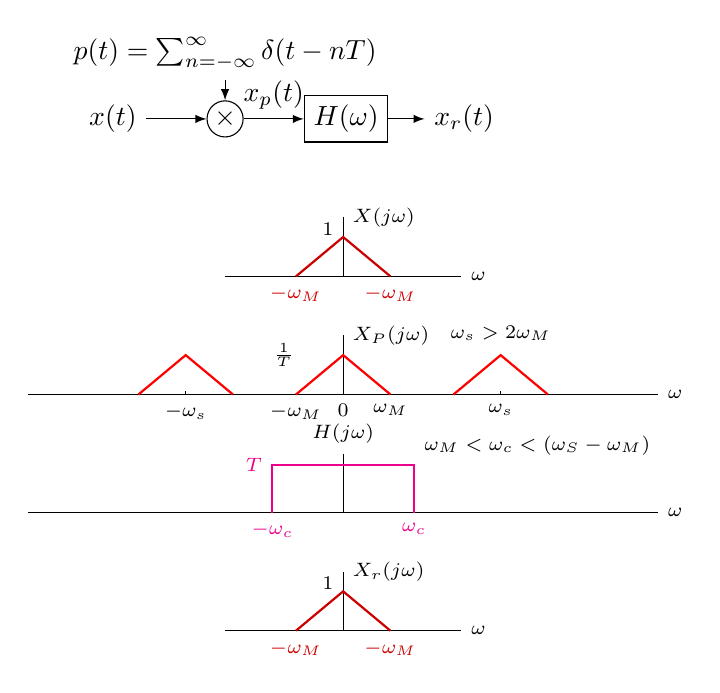
\begin{tikzpicture}[scale=0.5]
	\draw (0,0) node (a) [anchor=east] {$x(t)$} ++(2,0) node (b) [draw, circle, inner sep=1pt] { $\times$} ;
	\path (2,1) node (d) [anchor=south] {$p(t) = \sum_{n=-\infty}^{\infty}\delta(t-nT)$} ++(0, -2);
	\path  (b)  ++(2,0) node (c) [anchor=west, draw, rectangle, minimum height = 0.5cm] {$H(\omega)$};
	\path (c) ++(3,0) node (e) {$x_r(t)$};
	%\edge (a) -- (b);
	
	
	\draw[-latex]  (a) edge (b);
	\draw[-latex]  (b) edge node[above] {$x_p(t)$}(c) ;
	\draw[-latex]  (d) edge (b);
	\draw[-latex]  (c) edge (e);
    	\def\wm{1.2}
    	\def\ws{4.0}
    	\def\wc{3.6}

        \begin{scope}[yshift=-4cm, xshift=5cm]
            \draw (0,0) ++(-3,0) -- ++(6,0) node[anchor=west] {\scriptsize $\omega$};
            \draw (0,0) -- ++(0,1.5) node[anchor=west] {\scriptsize$X(j\omega)$};
            \draw[red!80!black, thick] (0,0) ++(-\wm,0) node[anchor=north] {\scriptsize$-\omega_M$} -- ++(\wm,1) -- +(\wm, -1) node[anchor=north] {\scriptsize$-\omega_M$};
            \node at (0, \wm) [anchor=east] {\scriptsize $1$};
        \end{scope}   	

        \begin{scope}[yshift=-7cm, xshift=5cm]
	        \draw (0,0) ++(-8,0) -- ++(16,0) node[anchor=west] {\scriptsize $\omega$};
	        \draw (0,0) -- ++(0,1.5) node[anchor=west] {\scriptsize $X_P(j\omega)$};
	        \foreach \w/\l in { -1/-\omega_s, 0/0, 1/\omega_s}
	        {
	
	            \draw[red, thick] (\w*\ws, 0) ++(-\wm, 0) -- ++(\wm, 1) -- ++(\wm, -1);
	            \node at  (\w*\ws, 0) [anchor=north, color=black] {\scriptsize $\l$};
	            \draw (\w*\ws, 0)  -- ++(0, 0.1);
	        }
	        \node [anchor=north] at (-\wm, 0) {\scriptsize$-\omega_M$};
	        \node [anchor=north] at (\wm, 0) {\scriptsize$\omega_M$};	
	        \node [anchor=north] at (\ws, 2) {\scriptsize$\omega_s > 2\omega_M$};	
	        \node [anchor=east, xshift=-0.5cm] at (0, 1) {\scriptsize$\frac{1}{T}$};	     	


	\end{scope}	
	
        \begin{scope}[yshift=-10cm, xshift=5cm]
	        \draw (0,0) ++(-8,0) -- ++(16,0) node[anchor=west] {\scriptsize $\omega$};
	        \draw (0,0) -- ++(0,1.5) node[anchor=south] {\scriptsize$H(j\omega)$};

 \draw[thick, magenta] (-\wc/2, 0) node [anchor=north] {\scriptsize $-\omega_c$} --  ++(0, 1.2) node [anchor=east] {\scriptsize $T$}  -- ++(\wc, 0)  node [anchor=south west, black] {\scriptsize $\omega_M< \omega_c < (\omega_S - \omega_M)$} -- ++(0, -1.2) node [anchor=north] {\scriptsize $\omega_c$} ;

	\end{scope}	

	        \begin{scope}[yshift=-13cm, xshift=5cm]
            \draw (0,0) ++(-3,0) -- ++(6,0) node[anchor=west] {\scriptsize $\omega$};
            \draw (0,0) -- ++(0,1.5) node[anchor=west] {\scriptsize$X_r(j\omega)$};
            \draw[red!80!black, thick] (0,0) ++(-\wm,0) node[anchor=north] {\scriptsize$-\omega_M$} -- ++(\wm,1) -- +(\wm, -1) node[anchor=north] {\scriptsize$-\omega_M$};
            \node at (0, \wm) [anchor=east] {\scriptsize $1$};
        \end{scope}

\end{tikzpicture} 